\section{Architecture}
\label{idea-sec-architecture}

Here we present the IDEA architecture. Beginning with a formal problem
definition, we present a brief overview, and then describe each major system
component in detail.

\begin{figure}[t]
\label{idea-fig-arch}
\begin{center}
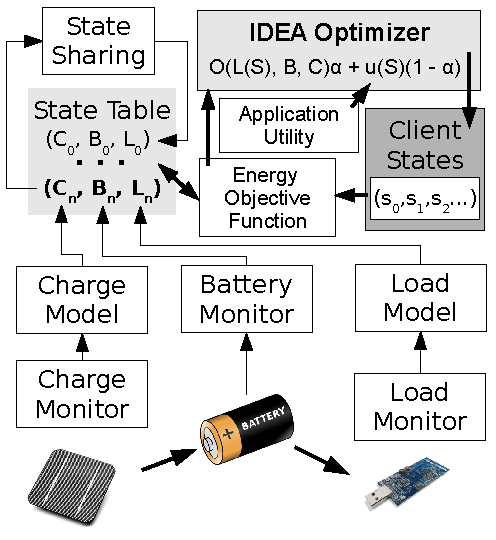
\includegraphics[width=\hsize]{./7-idea/figs/IDEAArchitecture.pdf}
\end{center}
\caption{\textbf{Overview of IDEA architecture.}
IDEA combines load and charge monitoring and modeling, energy state
distribution and an application-provided energy objective function into a
single service which can easily be integrated into application components.
Client states are evaluated by the energy objective function and also
assigned an application utility. These scores are combined by the optimizer
to select the state best balancing the application's distributed energy goals
against the state's intrinsic desirability.}
\end{figure}

\subsection{Problem definition}

IDEA is intended to address the problem of energy-aware tuning in
sensor network applications. In IDEA, we use the term {\em client} 
to refer to either a high-level application (such as a tracking system) 
or an individual software component that wishes to perform energy tuning 
(such as a MAC, routing, or time synchronization protocol). Clients
interact with the IDEA runtime residing on each sensor node 
to make decisions that impact energy consumption and data fidelity.

Sensor network software components commonly operate by making local
decisions. For example, many routing protocols form a spanning tree by each
node picking a parent based on local information, such as the radio link
quality or number of hops to the sink.  Likewise, duty-cycling MAC protocols
decide locally how often to poll the channel and check for traffic. In IDEA,
these choices are represented as a universe of possible {\em states}
$\mathcal{S}$ that the client can be in at any given time.  As an example, a
routing protocol's states represent the set of possible parents that the
protocol can choose. When using IDEA, the decision to switch to a given state
is based on a combination of the path quality (e.g., number of hops to the
sink) and the {\em distributed energy impact} of choosing a given parent.
Picking a given parent will impact the energy consumed by that parent as well
as nodes along the routing path from the parent to the sink. To be
energy-aware, the routing protocol must consider both the ``greedy''
desirability of a state (e.g., to maximize path quality) and its energy
impact.  Note that the ideal state may change over time, for example, based
on network load or energy availability. IDEA clients periodically reevaluate
their current state and may switch to a new state if it is deemed more
desirable.

IDEA is a sensor network service allowing clients to incorporate the {\em
distributed energy impact} of making local state decisions. By allowing
clients to estimate the \textit{global} energy impact of each state, IDEA
helps them make better \textit{local} decisions. IDEA quantifies the
distributed energy impact of each state using an application-defined
\textit{energy objective function}.  Each state $s \in \mathcal{S}$ produces
a energy load vector, $\bar{L}$, where each component $L_i^n(s_n)$ represents
the estimated energy load on node $i$ that will result from node $n$ setting
its local state to $s_n$.  We represent the current battery level (in joules)
at node $i$ by $B_i$, and the current charging rate (in joules per second) at
node $i$ by $C_i$.

Formally, we can define the problem that IDEA is addressing as
follows. At a given time, define the global state of all nodes
in the network as $S = \{ s_1, s_2, \ldots, s_k \}$.
The combined energy load at node $i$ induced by this selection of
states is
\[ L_i(S) = \sum_{j=1}^k L_i^j(s_j) \]
Based on the current
battery levels $B_i$ and charging rates $C_i$, we can define an 
{\em energy objective function} $O(\bar{L}(S), \bar{B}, \bar{C})$ that represents
the global energy impact of the state assignment $S$.
Likewise, each state assignment $S$ has an associated 
application-defined {\em utility} $u(S)$ that represents the
intrinsic desirability of the state --- for example, minimizing path
length in a routing protocol. 

The system's goal is to determine the optimal state 
\[
S^\star = \arg \max_{S} O(\bar{L}(S), \bar{B}, \bar{C}) \cdot \alpha + u(S) \cdot (1-\alpha)\]
where $\alpha$ represents the tradeoff factor between energy impact and
intrinsic utility. Setting $\alpha=1$ optimizes only for energy;
$\alpha=0$ only for application-defined utility.

\subsection{Energy objective functions}
\label{idea-subsec-energyobjectivefunctions}

Before describing the IDEA system itself, we first consider the space
of energy optimization goals that the system can target.
We expect that different applications will perform
energy allocation differently, and the objective function allows
the behavior of IDEA to be tuned to meet a variety of needs. 
Examples of possible objective functions include:
\begin{itemize}
\item \textbf{Maximize first-node lifetime.} Depending on energy load
and availability,
different nodes may run out of energy at different times. Given the
current load and charging rates, one can estimate the projected lifetime of
each node $i$ given global state $S$ as 
\[
\mathrm{T}(i,S) = \left\{ \begin{array}{lr}
\frac{B_i}{C_i - L_i(S)} & C_i < L_i(S) \\ \infty & C_i \ge L_i(S)
\end{array} \right. \] 
To maximize the first-node lifetime, we find the state $S^\star$ 
maximizing $O = \min_{i} T(i,S)$. This objective
function will always choose states that shift load away from the node
projected to die first, irrespective of the load that is produced on other
nodes, and may be suitable for applications whose fidelity requirements are
sensitive to the loss of single nodes.

\item \textbf{Maximize aggregate charging rate.} 
Given the charging rate $C_i$, battery level $B_i$ and battery capacity $P_i$
on node $i$, the effective charging rate given global state $S$ is
\[\mathrm{A}(i,S) = \left\{ \begin{array}{lr} C_i - L_i(S) & B_i \le P_i \\ 0 & B_i = P_i
\end{array} \right. \]
This reflects that when the node's battery fills it is no longer able to
collect charge. By maximizing $O = \sum_{i} \mathrm{A}(i,S)$, we
choose that state that leads to the network collecting charge as quickly as
possible.  When node batteries are all still charging this objective function
will try and find the state minimizing the total system load. However, once
batteries begin to fill, it will choose states that shift load towards nodes
charging full batteries, since any additional charge these nodes capture
cannot be stored. Shifting load towards overcharging nodes allows nodes
without full batteries to charge more rapidly. This objective function
prioritizes collecting charge over preserving node uptime, and may be
well-suited to applications that expect to experience periodic charging
cycles and can tolerate some nodes running out of energy.

% 11 Dec 2009 : GWA : Removing this to save space. Not sure it's needed.
%\item \textbf{Match load and charging rates.} 
%Another approach is to minimize the degree of energy imbalance in the sensor
%network, that is, to minimize $O = \sum_{i} \left| C_i - L(S)_i
%\right|$. This objective function tries to produce a load distribution
%matching the charging distribution.

\end{itemize}

One of the tradeoffs IDEA objective functions may perform is between
increasing the amount of charge collected --- which leads to reducing the
cumulative network-wide impact of each IDEA component --- and periods of node
downtime resulting from poor energy distribution.  Some applications may
weight node downtime differently for each node, depending on the quality of
the sensor data it is providing, its location, or other factors. Application
goals will differ, but the flexibility provided by the objective function
allows IDEA to support a variety of different requirements.

%Once each state has been scored by the energy objective function, the IDEA
%optimizer examines each state $s \in \mathcal{S}$, computing both the
%objective function $\mathcal{O}(\bar{v}(s))$ (calculated on the energy impact
%vector $\bar{v}(s)$) and the per-state utility $u(s)$. We seek a state
%balancing maximization of the objective function and per-state utility, with
%the tradeoff between the two parameterized by a weighting factor $\alpha$.
%Specifically, we seek to maximize $\alpha \cdot \mathcal{O}(\bar{v}(s)) +
%\left(1 - \alpha\right) \cdot u(s)$. $\alpha = 0$ means state assignment is
%done entirely on the basis of distributed energy impact; $\alpha = 1$ causes
%state assignment to be done entirely based on the components utility metric.

%Our current optimizer implementation enumerates all states $s \in
%\mathcal{S}$, performing an exhaustive search. For the applications we have
%explored to date the state space is small enough that this is feasible.
%However, we are exploring as future work the problem of searching state spaces
%that may be prohibitively large, or continuously parameterized.

\subsection{IDEA overview}

Thus far, we have defined the goal of the system as achieving a {\em globally
optimal} assignment of states $s$ to each sensor node.  Performing such a
global optimization would be possible through a central node (such as the
base station) collecting load and charge rates from every node and computing
the optimal assignment centrally, then informing all nodes of their states.
However, in large networks, this approach would induce large communication
overheads, reducing energy efficiency. Central control also precludes nodes
from making rapid local changes to states, for example, to select a new
parent in a routing tree if the current parent goes offline.

IDEA seeks to perform optimization in a {\em decentralized} fashion,
with the goal of closely approximating the globally optimal solution. An
important observation is that {\em most state changes only the impact energy
consumption of a node's immediate neighbors}.  Hence, nodes can perform a
local optimization using information gathered only from their neighbors.
Although this approach does not guarantee that the state assignment will be
globally optimal, we show in Section~\ref{idea-sec-evaluation} that it
approximates the optimal solution with low overhead.

Figure~\ref{idea-fig-arch} provides an overview of the IDEA architecture.
Each node {\em monitors} its own load rate, charging rate, and battery level.
Monitoring output is passed to a {\em modeling component} that produces
models of load and charging behavior.  Model parameters are distributed to
other nodes via a {\em state sharing} component, which maintains a state
table allowing energy information to be queried by energy objective
functions. IDEA monitors the accuracy of each node's local model parameters,
re-propagating them as necessary to maintain the accuracy of the distributed
energy information.

Clients periodically evaluate their current state, which can be driven either
by application-specific behaviors (e.g., disconnection from the parent node
in the routing tree) or changes to the energy state, triggered by IDEA. The
IDEA component residing on each sensor node evaluates the energy objective
function $O$ for each possible client state, which is combined with the
client utility function $u$ to determine the next state $s'$. In the
following sections we describe each component of the architecture in more
detail.

\subsection{Monitoring and modeling}

IDEA relies on the ability to measure and model load and charging
rates at each sensor node. This can be performed using either
hardware support, as in systems like Quanto~\cite{quanto-osdi08}, or
using software monitoring, as in Pixie~\cite{pixie-sensys08}. 
Modularizing these components allows IDEA to easily support multiple node
platforms and a variety of energy-harvesting hardware.

IDEA monitors both the energy load on a node as well as the charging rate,
both represented as joules per second. The battery level is monitored as
well. The raw measurements are used to build {\em models} that allow IDEA to
estimate the projected future energy load and availability. In addition, the
model parameters are distributed to other nodes in the network, allowing
those nodes to estimate the source node's energy load and charging profile
over time. 

IDEA provides a component that models load or charging rates by producing an
average across a fixed time window, which over time produces a piecewise-linear
model of varying load or charging rates. To estimate the load on a single
node $n$ at time $t$, $L_n(t)$, we compute $l_n = \frac{\int_{t - \Delta
t}^t \!  L_n(t)\, dt}{\Delta t}$, and distribute our estimate $l_n$ as the
single model parameter. This simple model must distribute new parameters to
incorporate time-varying load or charging rates. However, IDEA's modeling
architecture is modular and it would be straightforward to incorporate more
sophisticated charging models based on understanding of the underlying
dynamics of the energy harvesting technique being used. A seasonal ARIMA
model like that used by PRESTO~\cite{presto-TON} would provide more accuracy
when projecting future charging behavior.

%The monitoring and modeling stack is arranged as follows:
%\begin{itemize}
%\item \textbf{\texttt{CurrentMonitor}:} Provides the interface
%$\mathrm{getCurrent}()$ which returns $I(t)$, the current current.  Separate
%instances of this component are used to monitor load and charging rates.
%\item \textbf{\texttt{CurrentModel}:} Provides the interface
%$\mathrm{getParams}()$, which returns the parameter tuple $\mathbf{p} = {p_1,
%p_2, \ldots, p_i}$, and $\mathrm{useParams}(t, \mathbf{p})$, which returns an
%estimate of the current at time $t$ based on the provided parameter tuple.
%Separate instances model load and charging rates.
%\item \textbf{\texttt{BatteryMonitor}:} Provides the interface
%\texttt{getCapacity()}, which returns $B(t)$, the current battery capacity.
%\end{itemize}

IDEA distributes the battery state $B_n(t_0)$ at the time $t_0$ when it
updates the load or charging model parameters. To estimate the battery level
at time $t_1$, $B_n(t_1)$, we integrate the load and charging models, such
that $B_n(t_1) = B_n(t_0) + \int_{t_0}^{t_1} \! C_n(t) \, dt -
\int_{t_0}^{t_1} \! L_n(t) \, dt$.  Integrating the simple load model is
straightforward: $\int_{t_0}^{t_1} \!  L_n \, dt = \left( t_1 - t_0
\right) * l_n$. Other models may require more complex techniques.

We separate the modeling of load and charging rates for two reasons. First,
load and charging rates vary for different reasons: load fluctuates with
application demands, whereas charging rates fluctuate with environmental
variations. Disentangling energy inputs and outputs facilitates more accurate
modeling. Moreover, independent modeling of load and charging allows IDEA to
accurately model times when a node's batteries are exhausted. While a node is
running its overall current draw $I_n = C_n - L_n$. If $I_n > \beta$, where
$\beta$ is a threshold current necessary to enable battery recharging, then
the node is charging its battery; otherwise it is discharging. Once the node
dies, however, we assume that $L_n = 0$, and so $I_n = C_n$. Assuming future
energy inputs, a node that has completely drained its battery will be able to
recharge and rejoin the network once it has charged its battery past a
certain threshold.

Maintaining the accuracy of load and charging models on external nodes
requires periodically distributing updated model parameters. 
IDEA modeling components monitor the accuracy of the model they have
previously distributed. Using our simple linear model as an example, if
$l_n^{t_0}$ is the model parameter distributed for node $n$ at time $t_0$,
then at time $t_1$ the model will recompute $l_n^{t_1}$. If the relative
model error $\frac{\left| l_n^{t_1} - l_n^{t_0} \right|}{l_n^{t_0}} >
E$, where $E$ is an application-configurable error tolerance, then the
modeling component will push a new parameter to the state sharing layer,
which is responsible for updating other nodes.

\subsection{Distributed state sharing}

In order for nodes to make informed decisions about local state
changes, they must have knowledge of the energy profiles of other
nodes. IDEA provides a {\em state sharing} component that
automatically distributes local energy model parameters to
neighboring nodes, and collects model parameters from neighbors. This
is akin to the neighborhood communication model used in Abstract
Regions~\cite{regions-nsdi04} and Hoods~\cite{hoods-mobisys}. 

The distribution service maintains a local state table allowing estimated
energy information for other nodes --- including their battery levels
$B_i$, load rate $L_i$ and charge rate $C_i$ --- to be queried.
Estimates are produced by evaluating the load and charging models as
described previously.  Note that these values can be queried more frequently
than the underlying model parameters are updated.  The use of models allows
IDEA to significantly reduce the amount of communication and energy required
to distribute this information.

State sharing across nodes consumes energy, of course. However, our
evaluation shows that this overhead is recouped in improved overall energy
efficiency.  Without state sharing, nodes would be forced to make local
decisions about energy allocation that would underperform those made with the
benefit of limited state sharing.

IDEA provides a k-hop local state sharing implementation that disseminates
state updates using broadcast messages. We use a Trickle~\cite{trickle} timer
to balance rapid propagation of updates with eventual consistency in the face
of link failures. New updates cause the Trickle timer to be reset, causing
immediate state propagation. Nodes hearing the update relay it until the
maximum number of retransmissions is reached. We also utilize the broadcast
packets to opportunistically retransmit state for other nodes to reduce
propagation latency. When state retransmission is triggered a node fills
the broadcast packet with other recent updates from its state table.

IDEA clients frequently require propagating additional component-specific
state. A routing protocol may want to distribute what parents each node is
using, to allow a route through the network to be reconstructed. Nodes tuning
their own MAC parameters may need to distribute the parameters they are using so
that other nodes can communicate with them. Implementing component-specific
state sharing can be error-prone and produces additional energy consumption.
Instead, we have extended our state-sharing service to allow client code to
piggyback small amounts of application-specific state on the distribution
service. To simplify the implementation of the state-sharing service we limit
the amount of space available to client applications to ensure that the total
bundle of state fits within a single radio message.

\subsection{Client integration}

The interface between client components and IDEA is intended to
make it easy to integrate IDEA's runtime support for online energy
tuning into existing software. The IDEA optimizer provides an
interface, {\tt chooseState()}, that the client can invoke to select
a new state in an energy-aware fashion. Normally components may reexamine
state periodically to ensure that they respond to changes in network
dynamics. IDEA also provides event triggers that indicate when nearby energy
conditions have changed significantly, since these may also be opportunities
for clients to reevaluate their local state selection.
{\tt chooseState()} takes three arguments:
\begin{itemize}
\item A list of possible local states $s^n = \left\{ s^n_1, s^n_2, \ldots,
s^n_k\right\}$ that the client component on node $n$ can enter;
\item For each state $s^n_i$, the intrinsic utility $u(s^n_i)$ of that state,
represented as a scalar value; and
\item For each state $s^n_i$, a projected energy load vector $\bar{L}(s^n_i)$
representing the estimated energy impact (in terms of joules/sec) induced by
the node entering state $s^n_i$. $\bar{L}$ has one element for each of the
neighbors of the current node. 
\end{itemize}
IDEA combines this information with knowledge of energy load and availability
to determine the ideal state $s'$ that the node should enter based on the
weighted combination of the objective function $O$ and the utility $u$.  {\tt
chooseState()} returns the new state $s'$ selected by the optimizer.

In many cases it is straightforward to interface IDEA to existing code. As we
demonstrate in Section~\ref{idea-sec-casestudies}, IDEA has been used to add
energy awareness to the CTP~\cite{ctp-sensys09} routing protocol with minimal
code changes.  Existing software components can be supported by wrapping them
in code that estimates energy impact, enumerates states, and interfaces to
the IDEA service.
